\section{Introduction}
Monte Carlo methods estimate quantities by random sampling. We compare a
serial CPU baseline, OpenMP, local MPI processes, and CUDA on an RTX 5060
Laptop GPU. The research question is how stream assignment changes throughput
and statistical reliability. This is a comparative study, not a new algorithm.
Applications motivating the sampling pattern include uncertainty propagation,
transport simulation and numerical integration.

\section{Literature Review}
Counter-based generators support parallel stream generation~\cite{salmon}.
NVIDIA documents cuRAND Philox seed, subsequence and offset mapping~\cite{curand}.
Eight recent supporting sources are linked in the bibliography and cited here;
their arXiv versions are labelled as such.

MC/DC's GPU portability work and OpenMC's cross-vendor transport study
address portable execution of production transport~\cite{mcdc2025,openmc2024}.
Our CPU OpenMP implementation uses host threads, not OpenMP GPU offloading,
and our single GPU does not test cross-vendor portability.
MC/DC's event-processing comparison motivates attention to scheduling
in transport workloads~\cite{scheduling2025}; our fixed chunks and uniform
sampling do not reproduce those event queues.
The alternative to stride-based transport RNG highlights reproducible parallel
stream management~\cite{rng2024}; our chunk seeds and Philox subsequences
are practical mappings, not an implementation of that proposed method.

GPUmonty studies relativistic radiative transfer~\cite{gpumonty2026}, while
PUMI-Tally addresses unstructured-mesh tallies in OpenMC~\cite{pumi2025}.
These involve physics or mesh work absent from our small estimators, so
their bottlenecks and speedups are not transferable benchmarks.
GPU energy characterization in portable scientific applications provides
context for distinguishing power traces, workload scope and energy~\cite{energy2025};
our aligned GPU-only windows do not establish system-wide energy savings.
cuVegas uses adaptive importance and stratified sampling for multidimensional
integration~\cite{cuvegas2024}. Our uniform, separable known-answer integral
tests implementation and does not evaluate those variance-reduction methods.

This is a conceptual comparison, not a ranking of reported speedups.
\section{Problem Statement}
Generate uniform $(x_i,y_i)$ in the unit square and count
$H=\sum_i\mathbf{1}[x_i^2+y_i^2\leq1]$. The area is a quarter-circle, so
$p=\pi/4$ and $\widehat\pi=4H/N$. For independent points,
$\mathrm{Var}(\widehat\pi)=(4\pi-\pi^2)/N$.
CPU uniforms use $[0,1)$ and cuRAND uniforms use $(0,1]$;
the continuous targets agree, while finite-precision endpoints differ.
Extra literal digits cannot increase floating-point precision.

\section{Objectives}
Validate four programming models; measure total and GPU kernel time
separately; quantify stream-strategy effects on variance and interval
coverage; evaluate a known higher-dimensional integral; and collect scoped
GPU profiling and energy evidence on one laptop.

\section{Proposed Methodology}
CPU MT19937-64 streams belong to fixed chunks of 4096 samples, seeded using
experiment seed and chunk index. Thread/rank scheduling does not change
that mapping. Seed separation alone does not prove independence. CUDA uses
Philox subsequences indexed by global thread ID. The repeated-stream negative
control reuses CPU chunk streams or CUDA thread-index streams across blocks;
it is not a new RNG. CPU/GPU speedup compares implementations including
different RNG families, rather than hardware alone.

The common sweep uses two warm-ups and 30 measured trials per configuration;
the dedicated CUDA study uses three warm-ups, 100 CUDA run seeds and 30 serial
run seeds per configuration. Seeds are recorded and differ between replicates.
For sample values $Z_i$, shared code computes
\[
 \overline Z=\frac{\sum_i Z_i}{N},\quad
 s^2=\frac{\sum_i Z_i^2-(\sum_i Z_i)^2/N}{N-1}.
\]
\[
\mathrm{CI}_{95}\approx\overline Z\pm1.96\sqrt{s^2/N}.
\]
For pi, $Z_i=4\mathbf{1}[x_i^2+y_i^2\leq1]$, giving the corrected
standard error
\[\mathrm{SE}=4\sqrt{\widehat p(1-\widehat p)/(N-1)}.\]
The code clamps negative roundoff variance to zero. This is an approximate
normal interval, not an exact binomial interval: tiny samples or all-equal
outcomes may give a degenerate interval. Repeated streams violate its
independence assumption. Estimator variance and runtime dispersion are
separate quantities; empirical coverage does not prove RNG correctness.

\section{System Architecture}
Configuration supplies problem, sample count, experiment seed and backend
parameters. All four backends are implemented and produce sample moments;
shared code computes estimates, intervals and CSV output. OpenMP uses private
chunk engines and moment reductions. MPI distributes chunks among local
processes and reduces moments to rank zero. CUDA performs grid-stride sampling
and block reduction, followed by host accumulation of block results.


\begin{figure}[t]
\centering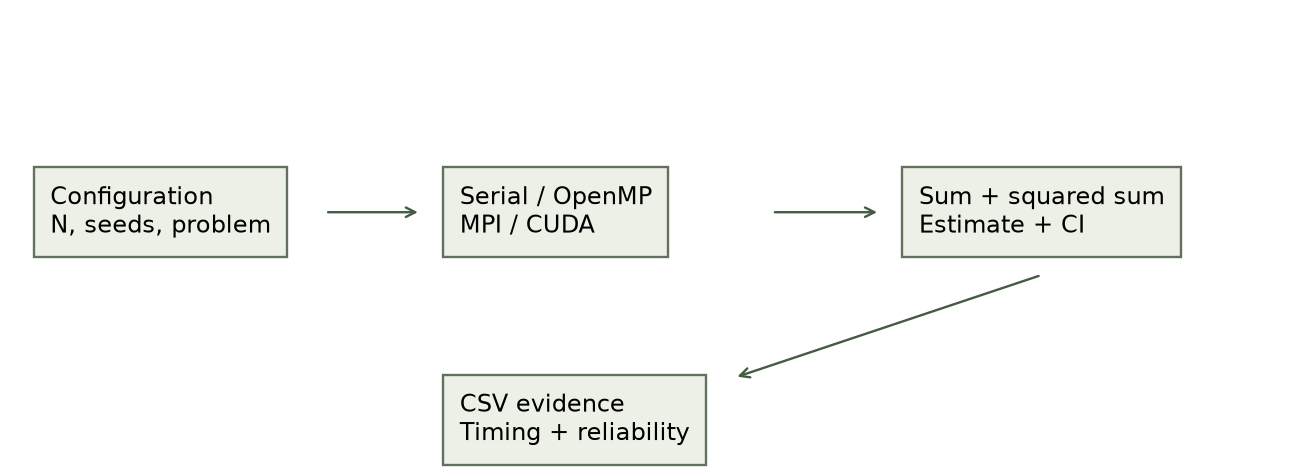
\includegraphics[width=\reportfigurewidth]{figures/architecture.png}
\caption{Shared configuration and statistical analysis across four execution paths.}
\end{figure}
\section{Algorithms}
Serial execution traverses chunks in order. OpenMP distributes chunk IDs with
a static work-sharing loop and reduces both moment sums. MPI rank $r$ owns
chunks $r,r+P,r+2P,\ldots$; ranks without work still enter the collectives.
Partial final chunks are bounded by $N$. CPU pi results preserve the sample
mapping across worker counts; integral sums can differ in their last bits
because floating-point addition depends on reduction order.
The higher-dimensional target is
\[
 I_d=\int_{[0,1]^d}\frac1d\sum_{j=1}^d x_j^2\,dx=\frac13,\qquad
 \mathrm{Var}(\widehat I_d)=\frac{4}{45dN}.
\]
This smooth separable average validates implementation across dimensions.
Its variance decreases with $d$ by construction; it does not demonstrate
overcoming the curse of dimensionality or a QMC advantage.

\section{Experimental Setup}
One Windows laptop, RTX 5060 Laptop GPU, driver 610.62, CUDA 13.3, MSVC 2026,
and Microsoft MPI runtime/SDK. The CPU is an Intel Core Ultra 7 255HX with 20 logical processors.
Configuration metadata records compiler and power-plan information;
continuous CPU thermal traces were not collected. Serial/OpenMP/MPI share optimization
settings. MPI processes run on one laptop, not multiple networked nodes.

OpenMP times parallel-region creation, sampling and reduction, and records
actual team size. MPI starts timing after a pre-trial barrier, includes local
sampling and moment reduction, and reports the maximum rank duration.
MPI startup, the barrier and the timing-metadata reduction are excluded.
CUDA events measure kernel time including RNG initialization and reduction.
Total CUDA trial time includes allocation, sampling, reduction, transfer,
host accumulation and device free. Context startup, event setup and process
launch are excluded. Host waiting overlaps GPU execution and must not be
added again to kernel time.

\section{Results}
Validation on 3 November 2026 confirmed OpenMP/MPI checks passed with 1, 2, 4 and 8 threads or local ranks,
both problems, both stream modes, and sample counts
2, 4095, 4096, 4097 and 100000. These cover empty ranks, chunk boundaries,
partial chunks, seed repeatability, interval agreement and invalid inputs.
Integral comparisons allow $10^{-12}$ for reduction-order differences.
These are recorded verification results, not a proof of RNG independence.

The common sweep completed 72 pi configurations and 24 eight-dimensional
integral configurations, with 30 trials each: 2880 measured trials.
Configuration order was fixed in a single session. Timing is exploratory;
apparent superlinear CPU speedups remain unvalidated.
The completed randomized follow-up contains 48 configurations,
three shuffled rounds of ten trials, or 1440 trials, with 30 distinct seeds
per configuration (round starting seed $12345+10r$).
At $N=10^7$ with separated streams, median total times were 108.1431 ms
for serial, 27.18275 ms for OpenMP with eight workers (3.978 times speedup),
32.35380 ms for MPI with eight ranks (3.3425 times), and 1.5904 ms for
CUDA with block 256 (67.997 times, including the RNG-family difference).
The earlier apparent eight-worker speedups above 10 or 14 times did not
reproduce. This strengthens the case against treating the fixed-order
superlinear observations as established scaling. It does not resolve every
timing issue: MPI with two ranks was slower than serial in the rerun.

The separate CUDA study on 28 October 2026 contains
60 CUDA configurations with 100 trials each and nine serial configurations
with 30 trials each (6270 observations), using a fixed shuffled configuration order, pi sizes
$10^4$ through $10^9$, and integral dimensions 2, 8, 16 and 32 at $N=10^6$.
At $N=10^9$, 512-thread blocks gave median total time 72.8308 ms and
kernel time 72.1121 ms. Small block-size differences do not establish a
decisive tuning advantage. At $N=10^8$, the largest matched median
implementation speedup was 174.90 times; CPU and GPU RNG families differ.

At $N=10^9$ with 256-thread blocks, separated CUDA streams gave
variance/theory 0.781 and coverage 98/100; repeated streams gave
162.268 and 12/100. Block-size configurations can share draws and must
not be pooled as independent replicates. Coverage uncertainty across seeds
is distinct from an individual estimate's interval.

Three completed, aligned sustained energy windows gave mean throughput
303097253 samples per GPU joule, approximately 303 million.
Timestamped power is integrated with boundary interpolation against reported
workload start/end times and completed trial counts. This is gross GPU-only
energy over the workload window, including host gaps and CSV output.
It is not per-kernel energy or CPU/whole-system energy.


\begin{table}[t]
\caption{Shuffled comparison: $N=10^7$, separated streams}
\centering\small
\begin{tabular}{lrrr}\toprule
Backend & Median (ms) & Speedup & CPU eff.\\\midrule
Sequential &108.1431&1.00&---\\
OpenMP (8)&27.1828&3.98&49.7\%\\
MPI (8)&32.3538&3.34&41.8\%\\
CUDA (256)&1.5904&68.00&---\\\bottomrule
\end{tabular}
\end{table}

\begin{figure}[t]
\centering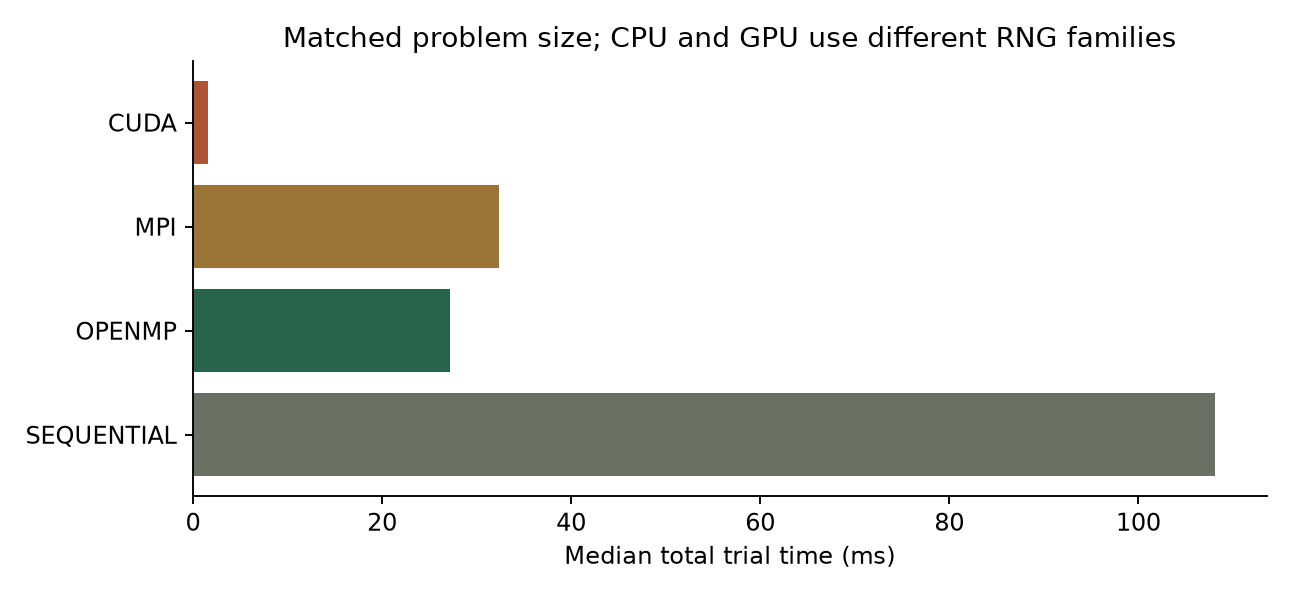
\includegraphics[width=\reportfigurewidth]{figures/backend_runtime.png}
\caption{Median total trial time in the shuffled comparison. CPU and GPU use different RNG families.}
\end{figure}

\begin{figure}[t]
\centering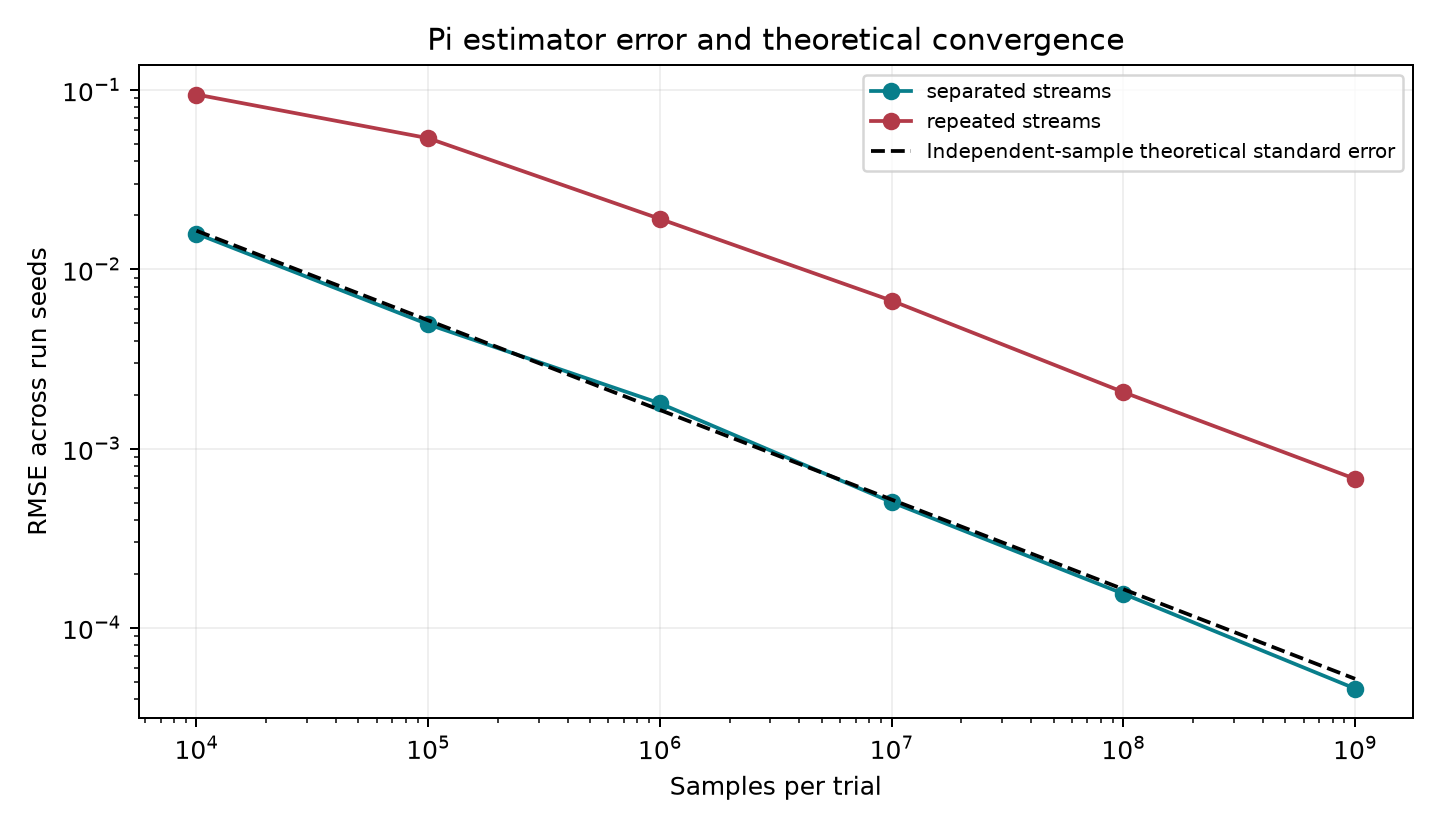
\includegraphics[width=\reportfigurewidth]{figures/accuracy.png}
\caption{RMSE across distinct seeds in the separate CUDA study. The theoretical line assumes independent samples.}
\end{figure}

\begin{table}[t]
\caption{Known integral: $N=10^6$, 100 CUDA trials per dimension}
\centering\small
\begin{tabular}{rrrr}\toprule
$d$ & Mean estimate & RMSE & Variance/theory\\\midrule
2 & 0.33332125 & 2.13e-04 & 1.024\\
8 & 0.33331805 & 9.55e-05 & 0.808\\
16 & 0.33332542 & 6.64e-05 & 0.791\\
32 & 0.33333530 & 5.06e-05 & 0.931\\
\bottomrule\end{tabular}\end{table}
\section{Performance Analysis}
Report means, medians, runtime dispersion and samples/second. CPU speedup is
$S=T_{\mathrm{serial}}/T_P$ and efficiency $E=S/P$ for threads or processes.
CUDA thread count is not a valid efficiency denominator. Values above
100\% efficiency can arise from cache effects, changing clocks, scheduling,
baseline variability or timing differences. The fixed-order common sweep
does not establish which explanation applies. The randomized follow-up did
not reproduce the earlier eight-worker superlinear observations; remaining
anomalies, including the two-rank MPI slowdown, need further investigation.

Counter-backed profiling is complete for the recorded configurations.
Nsight Compute requested base clocks and used replay, with one profiled
launch per configuration after three warm-ups. Pi at $N=10^8$ and $10^9$
achieved approximately 54 FP64 GFLOP/s against a clock-adjusted
126.36 GFLOP/s ceiling (42.7\%); the $d=8$ integral at $N=10^6$ achieved
78.06 against 126.28 GFLOP/s (61.8\%).
FP64 pipeline utilization was approximately 85--87\%, while rounded DRAM
throughput was at most 0.01\% of peak. Together these support an FP64
arithmetic bottleneck for these configurations, not every Monte Carlo kernel.
Pipeline utilization is not the percentage of peak FLOPs: the instruction
mix and fused operations affect those quantities differently.

Measured FLOPs count DADD + DMUL + twice DFMA; integer Philox work is excluded.
The tiny measured DRAM denominator makes arithmetic intensity sensitive
to cache state and background traffic. Replay/base-clock timings do not
replace unprofiled benchmarks, and one launch does not provide repeated-profile
confidence intervals. Profiling settings and counters are recorded with the experiment artifacts.
Power telemetry is coarse and may be hardware-averaged; CPU energy was not
measured, so no CPU/GPU energy-efficiency comparison is supported.
Floating-point precision and reduction roundoff are distinct from Monte Carlo
sampling error; faster execution alone does not improve statistical accuracy.


\begin{figure}[t]
\centering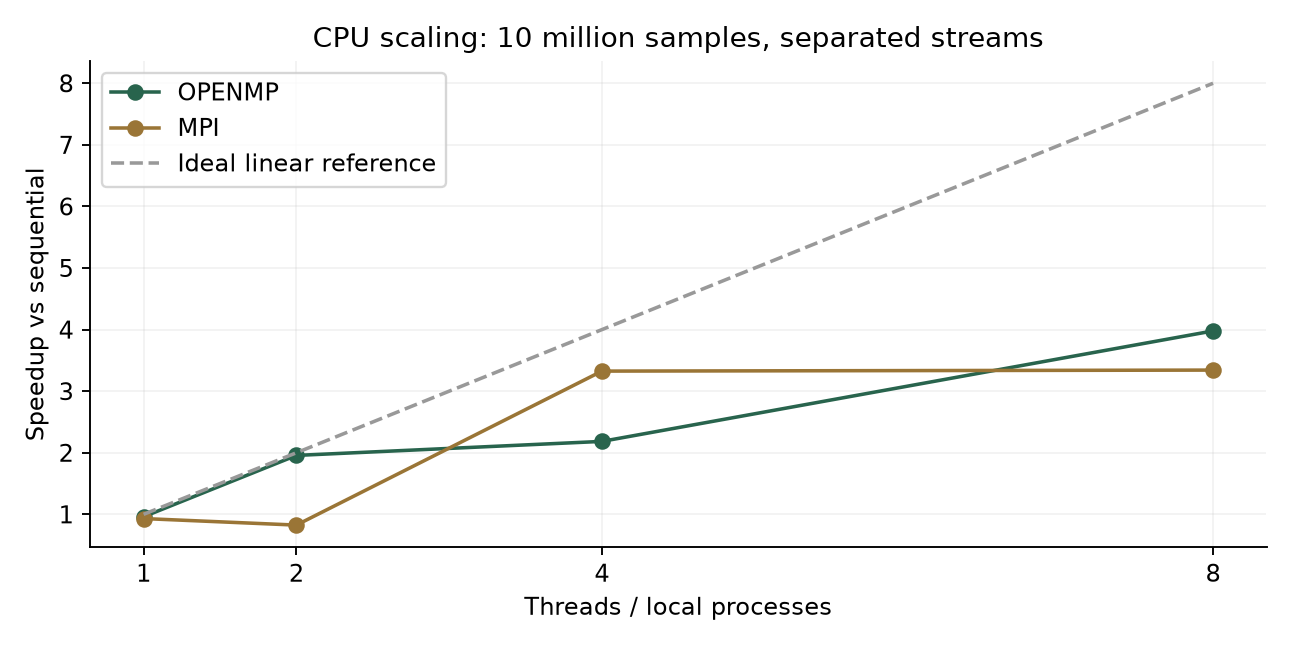
\includegraphics[width=\reportfigurewidth]{figures/cpu_scaling.png}
\caption{Local CPU scaling in the shuffled comparison; MPI uses one laptop.}
\end{figure}

\begin{figure}[t]
\centering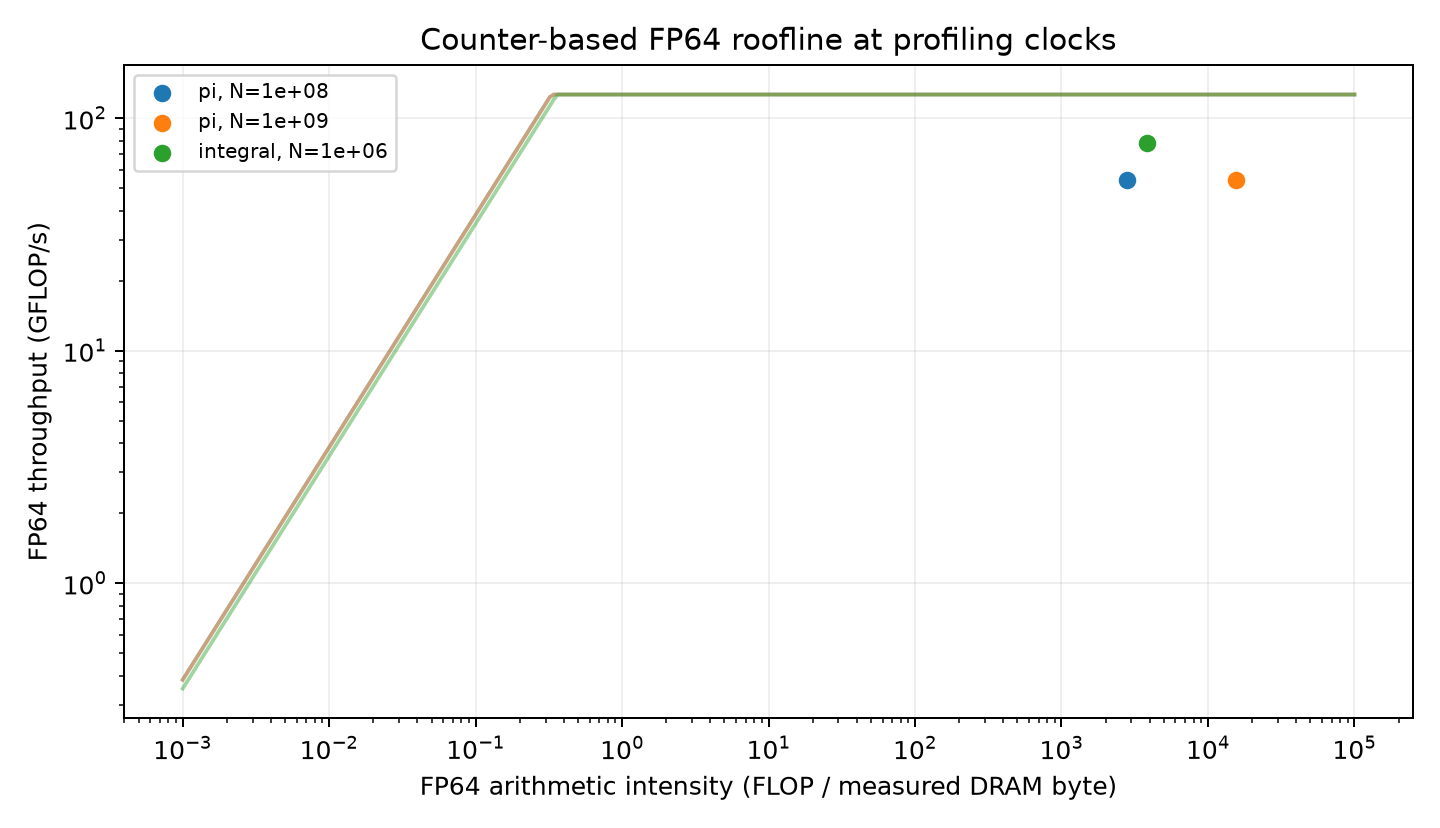
\includegraphics[width=\reportfigurewidth]{figures/roofline.png}
\caption{Measured FP64 roofline at profiling clocks. Integer RNG work is excluded from the FLOP count.}
\end{figure}
\section{Comparison with Existing Methods}
Published ratios use different workloads and baselines; none is a direct
ranking against our 68.00-fold implementation speedup.
Morgan et al. report C5G7 times of 5080 s on 112 CPU cores and 342.6 s
on four V100s (Table 1), approximately 14.83-fold acceleration~\cite{mcdc2025}.
Tramm et al. report 97\%, 96\% and 99\% weak-scaling efficiencies for
Aurora, Polaris and Frontier (Fig. 3), whereas our eight-worker CPU values
are strong-scaling efficiencies on one laptop~\cite{openmc2024}.
Cuneo et al. observe approximately $6.9\times10^5$ transport histories/s
with both scheduling methods at saturation (Sec. 5.1); histories involve
physics work absent from our point samples~\cite{scheduling2025}.

Cuneo and Variansyah compare stride/hash RNG runtimes of 113.26/111.46 s
and 1000-batch tally distributions (Sec. 5). Their normality tests and our
interval-coverage tests assess different statistical properties~\cite{rng2024}.
GPUmonty's laptop case reports 332 s on an RTX 3050 versus 2692 s on a
Ryzen 5 6600H (Sec. V.1); its register-related limits differ from our
FP64 diagnosis~\cite{gpumonty2026}.
PUMI-Tally reports at most roughly a twofold difference between its CPU
and GPU paths (Sec. 6, Fig. 4), emphasizing algorithm and data-layout
benefits beyond accelerator choice~\cite{pumi2025}.

Godoy et al. report 6--25\% mixed-precision QMCPACK energy savings
(Sec. 4.1, Table 3). Our 303 million samples/GPU-joule is an absolute,
workload-specific rate, not a comparable saving~\cite{energy2025}.
cuVegas reports 278.4-fold acceleration over its default Vegas baseline
(Table 7), using adaptive integration and error-aware comparisons.
Our uniform known-answer integral does not implement its variance
reduction or reproduce that benchmark~\cite{cuvegas2024}.

\section{Conclusion}
All four implementations are available, with recorded parallel correctness
checks and a completed exploratory common sweep. CUDA benchmark, sanitizer,
profiling and aligned GPU energy evidence are available. Reused streams can
yield poor coverage despite large nominal sample counts.
The randomized follow-up moderates the earlier CPU speedup claims, but
remaining timing anomalies require controlled follow-up. These results
support a scoped implementation comparison rather than a universal hardware ranking.

\section{Future Scope}
Investigate remaining CPU timing anomalies with controlled repetitions,
expand independent seed
replicates, compare matched RNG families and investigate nonseparable
integration or QMC. Repeated profiles and broader hardware measurements would
test the scope of the current bottleneck diagnosis. CPU/system energy and
multi-node MPI scaling are outside the present measurements.
